\documentclass[authoryear,preprint,review,12pt]{elsarticle}

\usepackage{amssymb}
\usepackage{amsmath}
\usepackage{booktabs}
\usepackage{lineno}
\usepackage{hyperref}
\usepackage{graphicx}
\usepackage{placeins}
\usepackage{tikz}
\usetikzlibrary{arrows.meta, positioning, fit, backgrounds}

\journal{Computers \& Geosciences}

\begin{document}

\begin{frontmatter}

\title{strandline: a dependency-light Rust engine for satellite-derived
shoreline extraction and change analysis, benchmarked against CoastSat
along the coast of Chile}

\author[1]{Francisco Parra-O.\corref{cor1}}
\ead{francisco.parra.o@usach.cl}
\cortext[cor1]{Corresponding author}

\author[1]{Mauricio Mar\'in}

\affiliation[1]{organization={Departamento de Ingenier\'ia Inform\'atica,
            Universidad de Santiago de Chile},
            city={Santiago},
            country={Chile}}

\begin{abstract}
Satellite-derived shorelines have become central to coastal-change analysis, and
open Python tools such as CoastSat have made them widely accessible. These tools
democratised the method but do not scale: they are interpreted pipelines built on
a heavy, fragile dependency chain, and reprocessing thousands of kilometres of
coast over decades is slow and hard to reproduce. We present \textbf{strandline},
a dependency-light Rust engine that ports the CoastSat method --- water index,
pixel classification, class-balanced Otsu threshold and sub-pixel marching-squares
contour --- into a single compiled binary and extends it with a native harmonic
tidal-correction synthesis, vectorised and parallel transect intersection, and
full DSAS-style change rates with quality control. Each stage is validated against
its reference: classification to within $1.5\%$ of CoastSat pixel-wise, tidal
prediction to $1.15$~mm against \texttt{pyTMD}, and transect intersection, rates
and quality control to rounding against a national erosion study. On matched
scenes the engine reproduces the CoastSat shoreline to a median of $0.2$~m,
while the transect-intersection step runs about $280\times$ faster than the
vectorised Python reference on the same computation ($37\times$
single-threaded) and the whole tool installs in one command. Across a
six-site benchmark spanning $24^\circ$ of latitude along the coast of Chile we
also report two findings with deliberately bounded claims. First, the geometry
along which a shoreline is refined is a separate choice from the geometry along
which its change is measured: refining the contour on normals derived from each
scene lowers the median error by about a fifth against the raw contour, whereas
fitting along the fixed transects helps only where they remain close to
shore-normal. Measured against an explicit null on an ocean-anchored transect
set, that misalignment is small (median $6^\circ$, a rate inflation below 1\%)
except at a migrating river mouth ($22^\circ$); on transects whose reference had
drifted inland, the same measurement returns a spurious $40^\circ$ that passes
tests of spatial coherence and temporal stability. Second, inter-sensor
precision, on which weighted change rates depend, is site dependent and smaller
than the fixed weights in common use assume, and must be calibrated and
validated per site. strandline removes the dependency and
performance barriers to satellite-derived-shoreline analysis at scale, and is
released open source with a citable archive.
\end{abstract}

\begin{highlights}
\item A single-binary Rust engine ports and extends the CoastSat SDS pipeline
\item Native harmonic tidal synthesis matches pyTMD to $\sim$1\,mm, no dependency chain
\item Vectorised transect intersection runs $\sim$280$\times$ faster than the Python reference
\item Median shoreline agreement with CoastSat $\sim$0.2\,m on matched Landsat scenes
\item Clean fixed transects sit $\sim$6$^\circ$ from shore-normal; drifted ones fake 40$^\circ$
\end{highlights}

\begin{keyword}
satellite-derived shorelines \sep coastal erosion \sep CoastSat \sep Rust \sep
tidal correction \sep shoreline change rates \sep DSAS \sep Chile
\end{keyword}

\end{frontmatter}

\linenumbers

%============================================================
\section{Introduction}
%============================================================
Sandy coastlines concentrate population, infrastructure and ecological value, and
they move: quantifying how shorelines have changed over decades is a prerequisite
for erosion management, hazard assessment and coastal planning. The satellite
record --- four decades of Landsat and, since 2015, Sentinel-2 --- has turned this
from a survey problem into an image-analysis problem, and a family of open tools
now extracts shorelines from that record at sub-pixel accuracy. Foremost among
them is CoastSat \citep{vos2019coastsat}, a Python toolkit that couples a
pixel classifier, a thresholded water index and a marching-squares contour to
produce georeferenced, tide-correctable shorelines, and which has become the
de-facto standard; CoastSeg \citep{fitzpatrick2024coastseg} builds a browser-based
hub around it and the Doodleverse segmentation models, and the SHOREX/SAET line
\citep{pardopascual2018shorex,palomarvazquez2023saet} offers an alternative
sub-pixel extraction validated on Mediterranean beaches. A community benchmark now
places the achievable accuracy of these methods at roughly $7$--$10$~m
\citep{vos2023benchmark}.

These tools democratised satellite-derived shorelines, but they share an
architecture that becomes a bottleneck at scale. All are Python pipelines built on
a heavy, fragile dependency chain --- GDAL bindings for I/O, scikit-learn for
classification, and, for tidal correction, packages such as \texttt{pyfes} or
\texttt{pyTMD} that are themselves awkward to install. In building a national,
$40$-year erosion assessment for the coast of Chile
\citep[][in review]{parra_erosion} we met the consequences directly: CoastSat's
per-transect \texttt{compute\_intersection\_QC} took over twenty minutes for a
single site of $\sim$180 transects against $\sim$800 shorelines; the tidal
dependency existed only on one packaging channel and forced a mid-project
migration; and reproducing the environment required source patches to the library
itself. None of these is a flaw in the science of the method --- they are costs of
the implementation, and they compound when the target is a thousand kilometres of
coast processed over four decades.

A natural response is a compiled engine: a single self-contained binary with no
interpreter and no dependency resolution, parallelised across cores, that performs
the same computation faster and installs in one step. This is the approach we have
taken for other geoscientific workloads \citep[][in review]{surtgis}, but for
satellite-derived shorelines no compiled tool exists --- to our knowledge the
entire field is Python. There is thus an open niche for a challenger that is
faithful to the established method yet built for scale, and a clear yardstick
(CoastSat) to validate it against.

We present \textbf{strandline}, a dependency-light Rust engine for
satellite-derived shoreline extraction and change analysis. It ports the CoastSat
method faithfully --- the same water index, the same classifier weights, an
equivalent sub-pixel contour --- and validates each stage against CoastSat,
\texttt{pyTMD} and the stored outputs of the Chilean erosion study, so that its
speed is never bought with a change in result. It then adds three things the
Python ecosystem provides only through external dependencies or not at all: a
native harmonic tidal synthesis that removes the \texttt{pyfes}/\texttt{pyTMD}
requirement, a vectorised and parallelised transect-intersection and change-rate
stage, and native coordinate transforms and cloud handling. Concretely, this paper
contributes:

\begin{enumerate}
  \item a faithful, single-binary Rust port of the CoastSat extraction pipeline,
  validated pixel- and metre-wise against the reference (Sects.~\ref{sec:data}--\ref{sec:results});
  \item a native harmonic tidal-correction synthesis, agreeing with \texttt{pyTMD}
  to millimetres, that eliminates the tidal dependency chain (Sect.~\ref{subsec:tide});
  \item a vectorised, parallel transect-intersection and DSAS change-rate stage
  that reproduces the reference exactly while running roughly two orders of
  magnitude faster (Sect.~\ref{sec:results});
  \item a separation of the geometry used to refine a shoreline from the
  geometry used to measure its change, and a direct measurement, against an
  explicit null, of how far fixed transects depart from the local shore-normal:
  little on clean geometry, substantially at a river mouth, and spuriously much
  where the transect reference has drifted inland
  (Sects.~\ref{subsec:geom}--\ref{subsec:angle});
  \item a six-site benchmark spanning $24^\circ$ of latitude along the coast of
  Chile, comparing accuracy, speed and installation footprint against CoastSat
  (Sects.~\ref{sec:data}--\ref{sec:results}).
\end{enumerate}

\noindent The remainder of the paper describes the engine and its validation
(Sect.~\ref{sec:engine}), the study sites (Sect.~\ref{sec:data}) and benchmark
design (Sect.~\ref{sec:methods}), the results (Sect.~\ref{sec:results}), and their
implications and limits (Sects.~\ref{sec:discussion}--\ref{sec:limitations}).

%============================================================
\section{The strandline engine}\label{sec:engine}
%============================================================
strandline is a Rust workspace of two crates: a library, \texttt{strandline-core},
that holds all numerical logic, and a command-line binary, \texttt{strandline-cli},
that exposes it as eleven composable subcommands: \texttt{fetch} for
acquisition, \texttt{extract}, \texttt{profile} and \texttt{baseline} for
shoreline extraction, \texttt{transects} and \texttt{intersect} for the
measurement geometry, \texttt{tide} and \texttt{rates} for correction and change
rates, and \texttt{slope}, \texttt{stl} and \texttt{satellite-weights} as
analysis tools. Pixel classification and quality control are not separate
subcommands but flags of the stages they belong to (\texttt{extract
-{}-classify}, \texttt{rates -{}-qc}).
Raster input/output, coordinate-reference-system handling and
the underlying array substrate are provided by \texttt{surtgis-core}, a sibling
geospatial engine; every other operation described below is implemented natively,
so the compiled binary carries no Python, GDAL-binding or numerical-library
runtime dependency.

\subsection{Pipeline overview}
The reference workflow maps a multispectral scene to per-transect change rates in
a single directed chain (Fig.~\ref{fig:pipeline}): a georeferenced
GeoTIFF/COG is read and a water index computed; pixels are classified into
sand, water, whitewater and other; an adaptive threshold on the water index,
restricted to the classified beach, defines the land--water boundary; a sub-pixel
contour of that boundary yields the instantaneous shoreline; transects cast
perpendicular to a smoothed baseline are intersected with the shoreline time
series; the resulting cross-shore distances are optionally tide-corrected and
reduced to erosion/accretion rates with per-transect uncertainty; and a set of
quality-control criteria flags unreliable transects. Each stage is also a
standalone entry point, so the engine can be used as a full pipeline or as
individual, scriptable operators.

\begin{figure}[t]
  \centering
  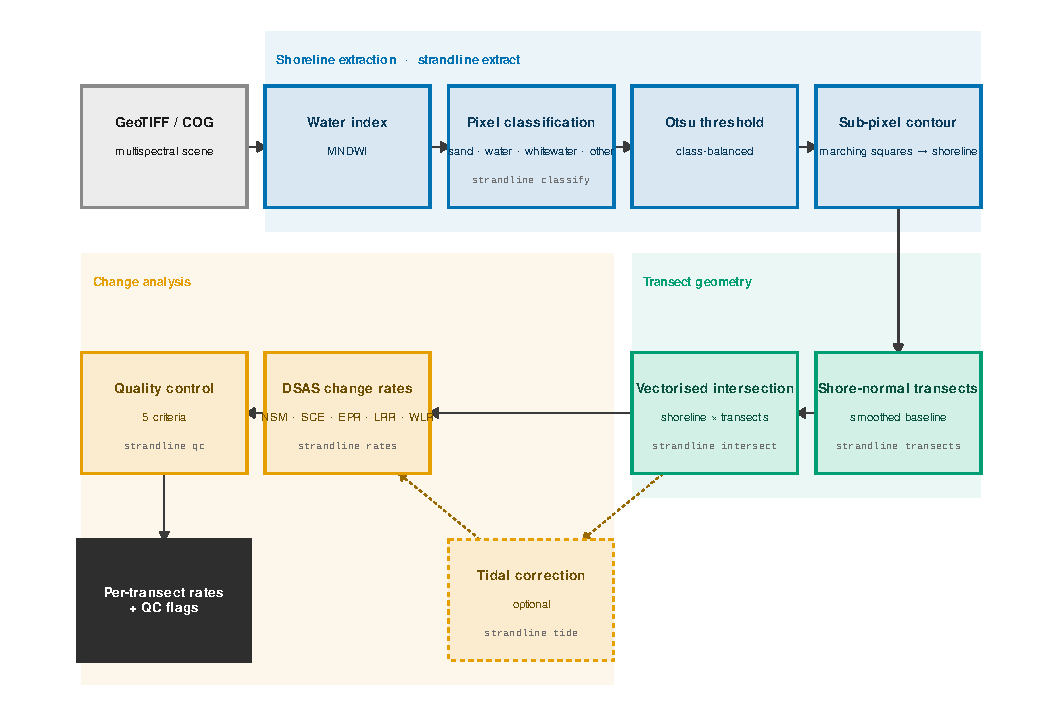
\includegraphics[width=\linewidth]{figures/pipeline.pdf}
  \caption{The strandline pipeline, grouped into three phases: shoreline
  extraction (blue), transect geometry (green) and change analysis (orange).
  Each box is a \texttt{strandline-core} operator, also exposed as the CLI
  subcommand shown in monospace. A multispectral scene enters top-left and the
  flow returns per-transect rates with quality-control flags at bottom-left. The
  tidal-correction step (dashed) is optional and applies to the cross-shore
  distances before rate fitting.}
  \label{fig:pipeline}
\end{figure}

\subsection{Water index and pixel classification}
The land--water contrast is captured by the Modified Normalised Difference Water
Index \citep{vos2019coastsat},
\begin{equation}
  \mathrm{MNDWI} = \frac{\rho_\mathrm{Green} - \rho_\mathrm{SWIR1}}
                        {\rho_\mathrm{Green} + \rho_\mathrm{SWIR1}},
  \label{eq:mndwi}
\end{equation}
computed together with the other normalised-difference indices used downstream.
Normalised differences are numerically fragile where the denominator approaches
zero: Landsat Collection~2 surface-reflectance products admit small negative
reflectances after atmospheric correction, and a handful of pixels where
$\rho_\mathrm{Green}+\rho_\mathrm{SWIR1}$ crosses zero can produce values of
hundreds to thousands rather than a bounded index, corrupting the downstream
histogram. The index routine therefore rejects (sets to \texttt{NaN}) any result
whose magnitude exceeds a guard value of $5.0$ --- large enough to pass genuine
but moderate excursions slightly outside $[-1,1]$ that the reference
implementation also tolerates, while removing true numerical blow-ups.

Pixels are classified with the same four-class multilayer perceptron distributed
with CoastSat. The trained scikit-learn weights are converted once to an embedded
JSON blob (52.9~kB) compiled into the binary, so classification requires no
Python or scikit-learn at run time. The 20-element feature vector replicates the
reference exactly: the five spectral bands, five normalised-difference indices,
and the $3\times3$ local standard deviation of each, computed \texttt{NaN}-aware
with reflect padding. A forward pass assigns each pixel its class, after which
small connected components are removed (8-connectivity) to suppress speckle. On a
held-out test scene the classified pixel counts agree with the CoastSat reference
to within $1.5\%$.

\subsection{Threshold and sub-pixel contour extraction}\label{subsec:threshold}
Within the sand-and-water region the land--water boundary is placed by an Otsu
threshold on the water index. Because the beach classes are typically imbalanced,
we use a class-balanced variant (\texttt{balanced\_otsu}) that weights the two
populations equally and is fully deterministic --- the reference implementation
balances the classes by random subsampling instead, and thresholds over a buffer
around a reference shoreline rather than the whole scene
(Sect.~\ref{subsec:divergences}). The shoreline is then extracted
as a sub-pixel contour of the thresholded index by a marching-squares algorithm
with linear interpolation along cell edges, reproducing the behaviour of
\texttt{skimage.measure.find\_contours}.

Cloud handling is explicit rather than incidental. The raw cloud mask is first
cleaned by removing small connected components (4-connectivity, minimum 40
pixels), which eliminates the false clouds that the CFMASK product places over
whitewater and that otherwise fragment the coast. Remaining clouds are then
buffered by a configurable distance (default 300~m) computed with an exact
Euclidean distance transform \citep[after][]{felzenszwalb2012edt}, and shoreline
polylines are split where they enter the buffer. Against the CoastSat shoreline
for the same scenes this cloud treatment improves the median point-to-line
agreement to $\approx0.20$~m and reduces coastal fragmentation substantially.

\subsection{Native tidal correction}\label{subsec:tide}
Tidal correction projects each instantaneous shoreline to a common datum along
the beach face \citep{vos2019coastsat}. Given a water level $\eta$, a reference
elevation $z_\mathrm{ref}$ and the beach-face slope $\tan\beta$, the horizontal
correction applied to a cross-shore distance is
\begin{equation}
  \Delta x = \frac{\eta - z_\mathrm{ref}}{\tan\beta},
  \qquad
  x_\mathrm{corr} = x_\mathrm{raw} - \Delta x .
  \label{eq:tide}
\end{equation}
Applied to the reference cross-shore distances this reproduces the paper's
tide-corrected series exactly.

The distinctive element is that water levels are synthesised natively, removing
the dependency on \texttt{pyfes}/\texttt{pyTMD} that motivated much of this work.
From a set of local harmonic constituents (the routine ships the thirteen
principal ones: $M_2, S_2, N_2, K_2, K_1, O_1, P_1, Q_1, M_f, M_m, S_\mathrm{sa},
S_a, M_4$) the engine evaluates the equilibrium tide using Doodson equilibrium
arguments and Schureman nodal corrections, with mean astronomical longitudes from
Meeus' series. Validated against \texttt{pyTMD} with GOT constituents, the phase
of the equilibrium argument $V_0$ agrees to $<0.01^\circ$ and the total predicted
level to a maximum error of $1.15$~mm for realistic central-Chile constituents.
We note that this millimetre accuracy is a property of the synthesis \emph{given}
correct constituents: the engine reads local harmonic constants from a CSV
(SHOA port constants, or values exported once from a global model); the accuracy
of any particular prediction is bounded by the constituents supplied, not by the
synthesis.

\subsection{Transect generation and vectorised intersection}
Transects are generated shore-normal to a baseline: the baseline is resampled by
arc length, its tangent estimated by central differences, and the outward normal
oriented seaward from a hint point, so that each transect runs from land to sea.
Generated from the reference shoreline this reproduces the transects of the
reference dataset to a maximum coordinate error of $0.0$~m.

Intersecting a shoreline time series with the transects is the step that
dominates the cost of the Python pipeline, where the original CoastSat
\texttt{compute\_intersection\_QC} is a per-transect Python loop. We reimplement
it as a vectorised, \texttt{rayon}-parallel operator: for each transect, shoreline
vertices within an along-transect strip are projected onto the shore-normal
direction to give candidate chainages, reduced by \texttt{NaN}-aware statistics,
and screened by the same quality-control tests as the reference (maximum standard
deviation, maximum range, minimum number of points, with an
\texttt{auto}/\texttt{max}/\texttt{nan} policy for multiple intersections).
Against the paper's vectorised Python implementation over 200 synthetic shorelines
$\times$ 250 transects (49{,}602 crossings) the two agree with zero mismatches in
the \texttt{NaN} pattern produced by the quality control and a maximum chainage
difference of $0.1$~mm. On the same problem the Rust operator computes the
intersections in $0.027$~s against $7.34$~s for the vectorised Python
reference, a $\approx280\times$ speed-up (Sect.~\ref{sec:results}); relative to
the original per-transect CoastSat loop the gap is larger still.

\subsection{Change rates and quality control}
From each transect's cross-shore time series the engine computes the standard
shoreline-change statistics: Net Shoreline Movement (NSM), Shoreline Change
Envelope (SCE), End-Point Rate (EPR), Linear Regression Rate (LRR, with
$R^2$ and 95\% confidence interval matching \texttt{scipy.stats.linregress}), and
the Weighted Linear Regression rate (WLR) from a closed-form $2\times2$ weighted
least-squares solve. Time is expressed in decimal years following the reference
convention, and an optional iterative despiking step removes isolated
outliers before regression. Against the reference \texttt{rates} table over 179
transects the statistics match to rounding: NSM/SCE/EPR to $\sim5\times10^{-5}$~m,
LRR/$R^2$/CI to $\sim10^{-6}$, and WLR to $\sim10^{-5}$~m\,yr$^{-1}$.

Quality control applies the five criteria calibrated in the reference study, in a
fixed order so that the reported reason is the first that fails: $|\mathrm{LRR}|
\le 5$~m\,yr$^{-1}$, $\mathrm{SCE}\le 500$~m, temporal span $\ge 20$~yr, at least
$50$ valid observations, and $R^2\ge 0.01$; retained transects are classified as
erosional, stable or accretional at a $\pm0.5$~m\,yr$^{-1}$ threshold. Reproducing
the reference labelling over the same 179 transects gives zero mismatches in both
the exclusion flag and the failure reason.

\subsection{Implementation, parallelism and reproducibility}
The engine is written in safe Rust and parallelised with \texttt{rayon}. Parallel
execution is a default feature that can be disabled to obtain a fully
deterministic single-threaded binary; where both modes exist their outputs are
bit-for-bit identical, so parallelism never changes a result. The classification
stage in particular fuses feature computation and MLP inference into a single
parallel pass (a \texttt{FeatureBank}) that avoids materialising the intermediate
$n\times20$ feature matrix, which is the main scaling win. Coordinate
transformations between UTM and geographic coordinates are implemented natively
with Karney's series to fourth order, agreeing with \texttt{pyproj} to below
1~mm including the negative-northing case produced by northern-hemisphere export
grids, so no PROJ installation is required. The current version is covered by 106
tests across the library, command-line and integration suites, including golden tests of the
full GeoTIFF-to-shoreline path and of the ported MLP against the original
scikit-learn outputs; the test suite passes in both parallel and single-threaded
configurations and the code is \texttt{clippy}-clean. Source, the compiled
crate and a reproducibility archive with a citable DOI are available
(Sect.~\ref{sec:availability}).

%============================================================
\section{Data and study areas}\label{sec:data}
%============================================================
We evaluate the engine on six sites spanning roughly 24 degrees of latitude
along the coast of Chile (Fig.~\ref{fig:sites}, Table~\ref{tab:sites}), from the
hyper-arid Atacama margin at Arica ($\approx$18.5$^\circ$S) to the macro-tidal
humid archipelago of Chilo\'e ($\approx$42.5$^\circ$S). The set was chosen to exercise the pipeline
across contrasting coastal settings --- desert, semi-arid, central microtidal
urban, river-mouth estuary, temperate estuary and archipelago --- and to include
two large subduction earthquakes whose coseismic shoreline jumps stress the
change-rate stage: the 2010 $M_w$~8.8 Maule event (Constituci\'on) and the 2015
$M_w$~8.3 Illapel event (Coquimbo). The sites are the same ones used in a
national coastal-erosion study \citep[][in review]{parra_erosion}, whose
processed CoastSat outputs and derived rates serve as the reference against which
we validate.

\begin{figure}[t]
  \centering
  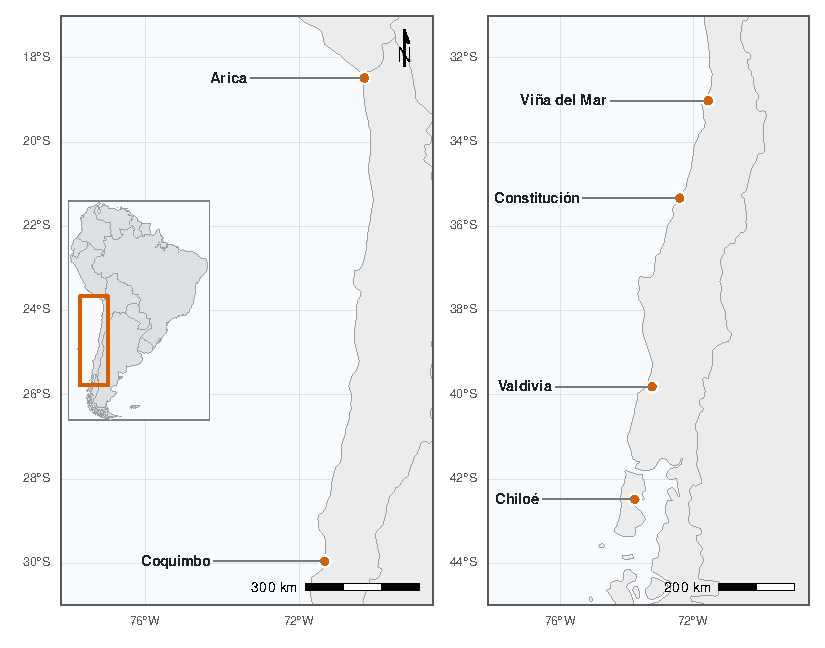
\includegraphics[width=0.86\linewidth]{figures/sites_map.pdf}
  \caption{The six benchmark sites along the coast of Chile, shown in a northern
  ($17$--$31^\circ$S) and a southern ($31$--$45^\circ$S) panel; the inset locates
  the study area within South America. The sites span desert, semi-arid, central
  microtidal, estuarine and macro-tidal archipelago settings, and include the
  2010 Maule and 2015 Illapel coseismic zones (Table~\ref{tab:sites}).}
  \label{fig:sites}
\end{figure}

Each site is a multidecadal time series of satellite-derived shorelines
(1984/1985--2025, $\approx$40~yr) built from the Landsat archive
(TM, ETM+, OLI/OLI-2; missions L5, L7, L8 and L9); Sentinel-2 is added at
selected sites for the streaming and inter-mission experiments
(Sect.~\ref{sec:results}). The number of usable scenes per site ranges from
392 (Coquimbo) to 1{,}228 (Constituci\'on), reflecting differences in cloud
climatology and revisit. Shore-normal transects are generated automatically from
a smoothed baseline at each site (100--334 transects, Table~\ref{tab:sites}).
Scenes enter the engine as multiband surface-reflectance GeoTIFFs; for the
streaming experiments they are read directly from Cloud-Optimised GeoTIFFs on a
public STAC catalogue without prior download.

The reference study derived each site's reference shoreline, and from it the
transects, from the detections themselves. A subsequent reanalysis of the same
sites found that at three of them (Vi\~na del Mar, Constituci\'on and Valdivia)
that reference had drifted into estuaries, lagoons or a river, so that most
retained transects did not sample the ocean shoreline, and that Coquimbo was
partially affected. The reanalysis anchors the reference to the OpenStreetMap
ocean coastline, re-extracts the shorelines restricted to within 300~m of that reference
(CoastSat's \texttt{max\_dist\_ref}), and
regenerates and orients the transects geometrically (95, 311, 118, 210 and 200
transects at Vi\~na del Mar, Coquimbo, Constituci\'on, Valdivia and Chilo\'e;
Arica, almost entirely on the open coast, was kept as processed). The two data
sets serve different purposes here. The equivalence checks of
Sect.~\ref{subsec:validation} use the stored tables of the original study,
because they test whether the port reproduces a given computation, which the
reference geometry does not affect. The geometric and inter-sensor analyses of
Sects.~\ref{subsec:geom}--\ref{subsec:satw} use the ocean-anchored reanalysis,
because they measure properties of the coast and the sensors that a drifted
reference would corrupt; Sect.~\ref{subsec:angle} shows by how much.

\begin{table}[t]
  \centering
  \small
  \caption{Study sites, ordered north to south. Scene counts refer to the
  satellite-derived shoreline time series, which spans 1985--2025 at every site
  except Chilo\'e, where it begins in 1984; transects are generated
  shore-normal to the site baseline. UTM zones are WGS84 south.
  $^\dagger$~Coseismic jump within the study period.}
  \label{tab:sites}
  \begin{tabular}{@{}lllrrr@{}}
    \toprule
    Site & Lat.\ ($^\circ$S) & Setting & UTM & Scenes & Transects \\
    \midrule
    Arica         & 18.5 & arid, desert            & 19S & 484 & 100 \\
    Coquimbo$^\dagger$ & 30.0 & semi-arid          & 19S & 392 & 334 \\
    Vi\~na del Mar & 33.0 & central, microtidal urban & 19S & 770 & 250 \\
    Constituci\'on$^\dagger$ & 35.3 & river-mouth estuary & 18S & 1228 & 176 \\
    Valdivia      & 39.8 & temperate estuary       & 18S & 753 & 334 \\
    Chilo\'e      & 42.5 & macro-tidal archipelago & 18S & 680 & 316 \\
    \bottomrule
  \end{tabular}
\end{table}

%============================================================
\section{Methods: benchmark design}\label{sec:methods}
%============================================================
The benchmark separates two questions that are often conflated: whether the
engine \emph{reproduces} the reference method (correctness), and whether it is
\emph{faster and lighter} while doing so (performance). We therefore validate
each stage against an independent reference before comparing run time, so that
speed is never bought with a silent change in output.

\subsection{Validation against the reference pipeline}\label{subsec:validation}
Each numerical stage is checked against the artefact that defines its correct
answer. The ported classifier is compared pixel-for-pixel against CoastSat on
held-out scenes and against the original scikit-learn network on golden feature
vectors. Transect generation, intersection, change rates and quality control are
checked against the reference study's stored per-transect tables: over the six
sites, generated transects reproduce the reference geometry to micrometres,
NSM/SCE/EPR match to $\sim5\times10^{-5}$~m and LRR/$R^2$/CI to $\sim10^{-6}$,
and the quality-control labelling reproduces the reference exclusion flag and
failure reason with zero mismatches. The tidal synthesis is validated against
\texttt{pyTMD} (Sect.~\ref{subsec:tide}). These are equivalence checks, not accuracy claims:
they establish that any downstream difference in a benchmark is attributable to
the engine's own choices rather than to a porting error.

\subsection{Documented divergences from the reference implementation}
\label{subsec:divergences}
A port whose value is fidelity should state where it is \emph{not} identical.
Auditing our implementation line-by-line against the CoastSat source
\citep{vos2019coastsat} identifies four deliberate divergences, all in the
extraction stage; none affects the transect, rate or quality-control results,
which reproduce the reference tables exactly (Sect.~\ref{subsec:validation}).
We list them so that residual differences in Sect.~\ref{sec:results} can be
attributed rather than absorbed.

\emph{Thresholding domain.} CoastSat computes the sand/water threshold using
only pixels inside the reference-shoreline buffer, dilated by five pixels, and
balances the two classes by random subsampling. strandline has no
reference-shoreline concept: it thresholds over the whole scene and balances the
classes deterministically by weighting rather than by sampling, so that the
result carries no dependence on a random seed. This is the most consequential
difference of the four: on scenes with abundant inland bright sand (dune fields,
dry river beds) the two samples genuinely differ, and part of the residual
disagreement reported in Sect.~\ref{sec:results} originates here rather than in
the contour arithmetic.

\emph{Pixels with undefined features.} CoastSat replaces every non-finite
feature value with $10^{-9}$ before classification, so a pixel whose local
standard deviation or spectral index is undefined --- typically deep shadow,
where an index denominator approaches zero --- is still assigned a class;
the subsequent test for remaining \texttt{NaN}s is unreachable. strandline
instead assigns such pixels to the \emph{other} class and excludes them from the
threshold sample. We prefer not to feed a placeholder value into a classifier
that was never trained on it, at the cost of a slightly smaller sample near
shadowed shorelines.

\emph{Low-sand fallback.} When fewer than 50 sand pixels fall inside the
reference buffer, CoastSat abandons the classifier-refined threshold and reverts
to a plain Otsu threshold on the water index. strandline has no equivalent
switch: with the classifier enabled it always uses the class-balanced threshold,
and the classifier-free mode is selected explicitly by the user rather than
triggered automatically. On scenes with almost no exposed sand --- a submerged
winter beach, an armoured urban front --- our threshold is therefore determined
by a small sand sample, and the classifier-free mode is the appropriate choice.

\emph{Proximity to nodata.} CoastSat discards shoreline vertices within a
hard-coded 30~m of any nodata pixel, in addition to the configurable cloud
buffer. strandline applies the same rule, with the threshold exposed as a
parameter defaulting to 30~m; nodata is identified from the bands exactly as in
the reference (any non-finite value, or Green, NIR and SWIR1 simultaneously
zero, the last being the signature of scene-edge fill and of scan-line gaps).
This matters most for ETM+ scenes acquired after the 2003 scan-line-corrector
failure, whose gap stripes cross the beach: without it, the vertices hugging
each stripe survive and feed the transect intersection.

Both this filter and the cloud buffer share one small numerical difference from
the reference: the distance is read from an exact Euclidean distance transform
sampled at the pixel nearest the vertex, whereas CoastSat measures the distance
from the fractional vertex position to each masked pixel directly. The effective
cut-off can therefore fall up to half a pixel diagonal ($\approx0.71$~px) below
the nominal one. At the 300~m cloud buffer this is immaterial; at 30~m it is
proportionally larger, and bilinear sampling of the distance field would remove
it.

\subsection{Accuracy against CoastSat}
Positional accuracy is measured as the agreement between a strandline shoreline
and the CoastSat shoreline for the \emph{same} scene, so that atmospheric,
tidal and acquisition effects cancel and the comparison isolates the extraction
method. For each pair we compute the symmetric point-to-line distance within a
fixed cross-shore corridor of 150~m and report its median, mean and 90th
percentile over the scene set. The CoastSat reference is generated with
pan-sharpening disabled, so that both engines read the same $15$~m raster and
the comparison is engine-against-engine rather than product-against-product.
Where strandline instead reads Landsat Collection~2 surface reflectance while
the reference remains top-of-atmosphere, we report the comparison as
inter-product ($30$~m SR against TOA on a $15$~m grid) and interpret the
residual accordingly; this sets a floor on achievable agreement that is
independent of the port.

\subsection{Speed, memory and installation}\label{subsec:speedmethod}
Run time is reported for the two stages that dominate cost --- the per-transect
intersection and the per-pixel classification --- in both the single-threaded
configuration and the default \texttt{rayon}-parallel one, against the
vectorised Python reference. As a proxy for deployment friction we also
contrast the installation footprint: a single \texttt{cargo install} producing
a self-contained binary versus a Conda environment resolving the CoastSat
dependency chain (GDAL, scikit-learn, \texttt{pyfes}/\texttt{pyTMD}).

Timings are wall-clock on an Intel Core i7-1270P (12 cores, 16 threads;
4 performance and 8 efficiency cores) with 38~GB of RAM under Linux, with
\texttt{rustc}~1.96.1 and NumPy~1.26.4, on a warm page cache. Each
configuration is measured over 21 repetitions of which the first three are
discarded, and we report the median with the interquartile range. Two design
choices matter for interpreting the result. First, the comparison is
computation against computation: the engine times only the intersection
operator, with the input parsed before the clock starts and the output
serialised after it stops, which is the counterpart of the Python function
operating on arrays already in memory; we additionally report the end-to-end
wall-clock of the command-line invocation, which includes process start-up and
CSV input/output and therefore penalises the engine rather than the reference.
Second, the repetitions are \emph{interleaved} rather than run in blocks, so
that a burst of unrelated load on the machine perturbs both sides of the ratio
equally. The second choice turns out to be the decisive one: the speed-up
ratio is markedly more stable than the absolute times it is built from. Two
independent runs whose median Python times differ by $13\%$ yield ratios that
agree to $0.1\%$. Ratios are therefore formed per repetition and summarised,
rather than taken as a quotient of medians, and a run is accepted only if the
interquartile range of every ratio stays within $20\%$ of its median --- a
criterion that rejects contended runs, where the dispersion of the reference
alone exceeded its own median.

%============================================================
\section{Results}\label{sec:results}
%============================================================
\subsection{Shoreline accuracy}
On matched scenes of the same product the engine reproduces the CoastSat
shoreline to sub-metre distances. Over six clear top-of-atmosphere scenes at
Vi\~na del Mar the median point-to-line agreement is $0.30$--$0.35$~m with the
classifier and CoastSat-compatible thresholding enabled, and improves to
$0.20$~m (mean $3.3$~m, 90th percentile $1.2$~m) once the cloud treatment of
Sect.~\ref{subsec:threshold} is applied; ranges span the two directions of the
symmetric point-to-line comparison. At these magnitudes --- a few hundredths of
the $15$~m grid the two engines share
--- the residual is dominated by the sub-pixel contour placement, not by any
systematic offset, confirming that the port reproduces the reference method
rather than merely approximating it.

Operating on surface-reflectance imagery read directly from the cloud, agreement
is coarser and set by product resolution rather than by the method: against the
top-of-atmosphere CoastSat reference a Landsat Collection~2 surface-reflectance
scene agrees to a median of $9.35$~m, an inter-product comparison of $30$~m
surface reflectance against top-of-atmosphere imagery on a $15$~m grid that amounts
to roughly $0.3$ native pixels and sits within the accuracy envelope reported for
satellite-derived shorelines by \citet{vos2023benchmark}. This surface-reflectance
figure, and how the geometry of the transect step moves it, is quantified across
all six sites in Sect.~\ref{subsec:geom}.

\subsection{Speed}
The vectorised, parallel operators reproduce the reference outputs
(Sect.~\ref{subsec:validation}) at a fraction of the cost. On the intersection benchmark ($250$ transects
$\times$ $200$ shorelines) the engine computes the intersections in $0.027$~s
against $7.34$~s for the vectorised Python reference, a $\approx280\times$
speed-up (Table~\ref{tab:speed}). The gap survives every way of drawing the
comparison: restricted to a single thread, so that it measures the port rather
than the parallelism, it is still $\approx37\times$; and charged with process
start-up and CSV parsing that the in-memory Python reference never pays, the
end-to-end command still returns in $0.13$~s, $\approx56\times$ faster.
Measured against the original per-transect CoastSat
\texttt{compute\_intersection\_QC} loop, which the reference study already
replaced because it took tens of minutes, the gap spans several orders of
magnitude.

\begin{table}[t]
  \centering
  \small
  \caption{Intersection benchmark, $250$ transects $\times$ $200$ shorelines,
  over 21 interleaved repetitions (first three discarded) on the hardware of
  Sect.~\ref{subsec:speedmethod}. The speed-up is formed per repetition and
  summarised, not taken as a quotient of medians. The first two rows compare
  the intersection operator against the equivalent Python function, both
  operating on data already in memory; the third charges the engine with
  process start-up and CSV input/output, which the reference does not pay.}
  \label{tab:speed}
  \begin{tabular}{@{}lrrr@{}}
    \toprule
    Configuration & Time (s) & Speed-up & IQR of speed-up \\
    \midrule
    Vectorised Python reference       & 7.34  & ---            & --- \\
    \midrule
    Intersection operator, 16 threads & 0.027 & $279.8\times$  & 15\% \\
    Intersection operator, 1 thread   & 0.201 & $37.2\times$   & 15\% \\
    End-to-end command line           & 0.132 & $56.3\times$   & 9\% \\
    \bottomrule
  \end{tabular}
\end{table} The classification stage, the other cost centre,
costs $\approx0.55$--$0.62$~s per scene single-threaded and $\approx0.15$~s on
16 cores; fusing feature extraction and inference into a single parallel pass,
rather than materialising the intermediate feature matrix, is what makes that
scaling possible, and it also lifted the stage from the $\approx0.9$~s of a
naive sequential implementation. Extraction with the classifier therefore
totals $\approx0.17$--$0.19$~s per scene, about $6\times$ faster than the
CoastSat classifier. Extraction without the classifier runs at $\approx18$~ms per scene
against $\approx1.17$~s for CoastSat ($\approx65\times$). Crucially the parallel
and single-threaded outputs are bit-for-bit identical, so these speed-ups change
only the run time, never the result.

\subsection{Native tidal synthesis}
The native harmonic synthesis matches \texttt{pyTMD} to millimetres: the phase of
the equilibrium argument agrees to $<0.01^\circ$ and the total predicted water
level to a maximum of $1.15$~mm over a realistic thirteen-constituent set for
central Chile --- a set that includes the annual solar constituent $S_a$, whose
astronomical argument is the one place where an error would otherwise pass
silently, since its long period leaves the shorter-period validation
unaffected. Applied to the reference cross-shore
distances, the horizontal correction of Eq.~\ref{eq:tide} reproduces the
reference study's tide-corrected series exactly.

The beach-face slope needed by Eq.~\ref{eq:tide} can itself be estimated from the
shoreline time series by minimising tidally-correlated residual energy. On
synthetic data with Landsat-like sampling the estimator recovers the true slope
to $\pm0.01$. On real data the picture matches the physical expectation: at
micro-tidal Vi\~na del Mar the slope is not identifiable from Landsat alone --- the
tidal signal is too small relative to sampling noise --- but a dense
Sentinel-2 series (215 scenes, 2019--2025, read from the cloud) makes it
identifiable, returning $0.097$ by direct regression, $0.105$ by the raw spectral
sweep and $0.073$ after robust despiking, against a literature value of $\approx0.10$.
Consistent with this, tidal correction does not reduce the \emph{aggregate}
shoreline-change envelope at Vi\~na ($\approx500$~m, dominated by multiple
intersections rather than tide); its effect is seen in the per-transect rates,
not in the envelope.

\subsection{Where the sub-pixel fit is sampled}\label{subsec:geom}
Both major satellite-derived-shoreline lineages measure change against a
\emph{fixed} geometry generated once from a historical reference line ---
CoastSat and the large-scale operational products cast fixed shore-normal
transects, and the SHOREX/SAET family deliberately reuses a single approximate
reference line for a whole image set for efficiency
\citep{pardopascual2018shorex,palomarvazquez2023saet}. For \emph{rates} this is
not merely conventional but necessary: a change rate is defined along a transect
that stays put, so the measurement geometry has to be stable across the series.
The question we can ask is therefore not whether to fix the transects, but
whether that same fixed geometry should also be used to \emph{refine} the
shoreline position within each scene.

The two roles come apart. A transect anchored to a past shoreline still
approximates the local shore-normal only as well as the coast has stayed put; on
a curved or dynamic coast it can meet the instantaneous shoreline at a
substantial angle. That is tolerable for a strip-based intersection, which only
needs to bracket the crossing, but not for a profile fit, whose window must
straddle the land--water edge along the direction of steepest change.

Table~\ref{tab:geom} separates the two roles on surface-reflectance scenes,
scored against the cross-shore distances of the ocean-anchored reanalysis
(Sect.~\ref{sec:data}). For each site we took Landsat~8/9 scenes from
2018--2021 with at most 15\% cloud cover whose date is also in the reference
series, up to 15 per site and spread over the period (90 scenes in all). All
three rows are measured along the \emph{same} fixed transects; what differs is
how the shoreline position is refined within each scene: not at all (the raw
marching-squares contour), by fitting a profile sampled along those same fixed
transects, or by refining the contour along short perpendiculars generated from
the scene's own contour. Refining on local normals gives the lowest median and
the widest coverage in both groups of sites: $12.5$~m against $16.0$~m for the
raw contour at the four sites with the most complex planform (Coquimbo,
Constituci\'on, Valdivia and Chilo\'e), a reduction of about a fifth, and
$10.2$~m against $12.3$~m at the two straight, stable ones (Vi\~na del Mar and
Arica). Fitting a profile along the fixed transects falls in between: it
improves on the raw contour at three of the four complex sites and at both
straight ones, and makes it worse only at Constituci\'on ($12.2$ against
$11.8$~m), the one site where the fixed transects are strongly misaligned
(Sect.~\ref{subsec:angle}). A finer estimator helps when it is sampled across
the edge and loses its advantage when it is sampled obliquely.

We read this as evidence that the geometry used to \emph{extract} a shoreline
and the geometry used to \emph{measure} its change are separate design choices,
and that only the second one has to be fixed: following each scene's own
contour is the more robust way to refine, and borrowing the measurement
geometry for that purpose costs accuracy precisely where that geometry has
drifted from shore-normal. The evidence is indirect, because it reads the
misalignment through its effect on a fitting window; Sect.~\ref{subsec:angle}
measures the angle itself. The comparison is also sensitive to the reference
geometry. Scored on the same scenes against the original, detection-derived
transects, the profile fit is worse than the raw contour at three of the four
complex sites ($14.7$ against $13.8$~m pooled), the ordering one would conclude
from those transects alone; on them the misalignment is much larger
(Sect.~\ref{subsec:angle}).

\begin{table}[t]
  \centering
  \small
  \caption{Shoreline position error (m) of three refinement strategies against
  the cross-shore distances of the ocean-anchored reanalysis, on the same 90
  surface-reflectance scenes (Landsat~8/9, 2018--2021, 15 per site).
  \emph{All three are measured along the same fixed transects}; what differs is
  how the shoreline position is refined. Lower is better; $n$ is the number of
  transect$\times$scene measurements. Complex: Coquimbo, Constituci\'on,
  Valdivia, Chilo\'e. Straight: Vi\~na del Mar, Arica.}
  \label{tab:geom}
  \begin{tabular}{@{}llrrrr@{}}
    \toprule
    Sites & Shoreline refinement & Median & Mean & P90 & $n$ \\
    \midrule
    Complex  & None (raw contour)                    & 16.00 & 95.84 & 369.09 & 4797 \\
             & Profile fit along the fixed transects & 13.90 & 64.19 & 181.61 & 8048 \\
             & Contour refined on local normals      & \textbf{12.46} & \textbf{54.60} & \textbf{134.07} & 9901 \\
    \midrule
    Straight & None (raw contour)                    & 12.28 & 98.11 & 460.44 & 980 \\
             & Profile fit along the fixed transects & 11.14 & 66.01 & 209.60 & 1577 \\
             & Contour refined on local normals      & \textbf{10.21} & \textbf{49.16} & \textbf{43.88} & 2252 \\
    \bottomrule
  \end{tabular}
\end{table}

\subsection{How far the fixed transects are from shore-normal}
\label{subsec:angle}
The previous section infers misalignment from its consequences. Here we measure
it on the ocean-anchored transects and the CoastSat shorelines re-extracted with
them --- no scene is re-processed by strandline and no comparison is made across
products, so the quantity is pure geometry.

The measurement matters because it is one-signed. A distance measured along a
transect that meets the shoreline at an angle $\theta$ from its local normal is
the true perpendicular distance divided by $\cos\theta$. If $\theta$ persists
for a given transect, the change rate inherits the same factor: a real
perpendicular retreat $\Delta$ registers as $\Delta/\cos\theta$. Because
$1/\cos\theta \ge 1$ always, misalignment can only inflate a rate, never deflate
it; transects tilted one way and the other inflate alike.

Estimating $\theta$ is less straightforward than it appears. The local
shore-normal has to be read off a marching-squares contour that is stepped at
pixel scale, so the estimator carries an error of several degrees. Worse,
$\theta = \arcsin|\hat{u}\cdot\hat{t}|$ is a \emph{rectified} quantity, so
estimator noise inflates the measured median even when the true angle is zero.
A low control value is therefore not enough; what is needed is a null
distribution. We build one by applying the identical estimator to the reference
shoreline from which the transects were generated --- where the true angle is
zero by construction --- resampled to the same vertex density as the
instantaneous contours and quantised onto the pixel grid to reproduce their
stepped structure. The signal is the excess over that null. Only the part of
the misalignment that persists for a given transect can bias its rate --- an
angle that varies randomly between dates adds variance but leaves the fitted
slope alone --- so we take, for each transect with at least 10 dates, the median
angle across dates and the spread about it.

The misalignment is small. Against a null whose site medians are
$1.3$--$4.1^\circ$, the measured angle has a median of $5.9^\circ$ (between $5.9$
and $8.0^\circ$ for estimator windows from $\pm60$ to $\pm200$~m), distinct
from the null ($p<10^{-15}$, Mann--Whitney, at every window) but only a few
degrees above it. The persistent component has a median of $5.7^\circ$ over 857
transects at five sites (Fig.~\ref{fig:angle}, Table~\ref{tab:angle}), which
corresponds to a median rate inflation of $0.5\%$; $17\%$ of transects exceed
$20^\circ$. The exception is Constituci\'on, where the transects cross the
mouth and spit of the Maule River: there the persistent angle is $22^\circ$
and the implied inflation $8\%$. Projecting each transect's published rate onto
its local normal would change the median magnitude by $0$--$10\%$ depending on
the site. Spatial coherence and temporal stability confirm that what remains is
geometry rather than noise: adjacent transects correlate at $r=0.36$--$0.74$
against permutation bands of at most $\pm0.22$, and angles computed on two
disjoint halves of the record agree at $r=0.77$--$0.98$.

\begin{figure}[!t]
  \centering
  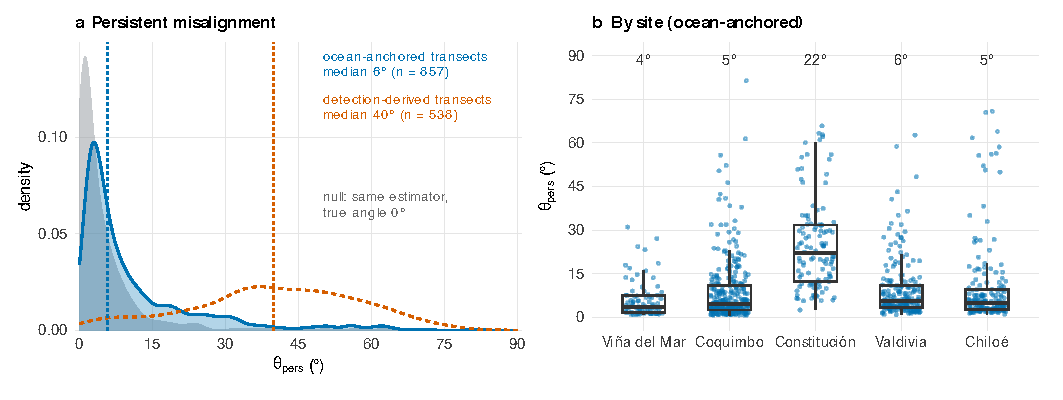
\includegraphics[width=\linewidth]{figures/transect_angle.pdf}
  \caption{Misalignment between fixed transects and the local shore-normal of
  the instantaneous shoreline. (a) Distribution of the persistent per-transect
  angle $\theta_\mathrm{pers}$ on the ocean-anchored transects (blue, five
  sites pooled) against the null obtained by applying the same estimator to a
  geometry whose true angle is zero (grey), and the same measurement on the
  detection-derived transects of the original study (orange, dashed), whose
  reference had drifted inland at three of the four sites. (b) Persistent angle
  per site on the ocean-anchored transects; the label gives the median. Only
  the Maule river mouth at Constituci\'on departs markedly from shore-normal.}
  \label{fig:angle}
\end{figure}

\begin{table}[t]
  \centering
  \small
  \caption{Misalignment between the ocean-anchored fixed transects and the local
  shore-normal of the instantaneous shoreline. $\theta_\mathrm{pers}$ is the
  per-transect median across dates (the component that can bias a rate); the
  fluctuating component is its median absolute deviation. Inflation is the
  median of $1/\cos\theta_\mathrm{pers}-1$. $r_\mathrm{space}$ is the
  correlation of $\theta_\mathrm{pers}$ between adjacent transects
  ($\approx$100~m apart) and $r_\mathrm{time}$ its correlation between two
  disjoint halves of the record. Every transect listed carries $\ge$10 dates.
  Arica is absent for lack of an archived per-date shoreline set.}
  \label{tab:angle}
  \begin{tabular}{@{}lrrrrrr@{}}
    \toprule
    Site & $n$ & $\theta_\mathrm{pers}$ & fluct. & inflation & $r_\mathrm{space}$ & $r_\mathrm{time}$ \\
    \midrule
    Vi\~na del Mar & 83  & 3.7$^\circ$  & 1.6$^\circ$  & 0.2\% & 0.62 & 0.86 \\
    Coquimbo       & 298 & 4.6$^\circ$  & 2.0$^\circ$  & 0.3\% & 0.43 & 0.96 \\
    Constituci\'on & 109 & 22.1$^\circ$ & 13.7$^\circ$ & 8.0\% & 0.74 & 0.77 \\
    Valdivia       & 192 & 5.7$^\circ$  & 2.6$^\circ$  & 0.5\% & 0.36 & 0.98 \\
    Chilo\'e       & 175 & 5.0$^\circ$  & 2.2$^\circ$  & 0.4\% & 0.56 & 0.98 \\
    \midrule
    All            & 857 & \textbf{5.7}$^\circ$ & 2.5$^\circ$ & \textbf{0.5\%} & & \\
    \bottomrule
  \end{tabular}
\end{table}

\paragraph{A drifted reference fakes a large angle.} The same measurement on the
original, detection-derived transects returns a very different picture: a
persistent median of $39.9^\circ$ over 538 transects at four sites, an implied
rate inflation of $30\%$, and spatial ($r=0.54$--$0.63$) and temporal
($r=0.76$--$0.93$) coherence of the same kind as above (Fig.~\ref{fig:angle}a).
Only 130 of those 538 transects (24\%) had their origin within 200~m of the
ocean coastline. Those that followed the bank of an estuary or a river measured
a real, persistent angle --- to the wrong shoreline --- and so passed both tests,
which can separate geometry from estimator noise but not ocean geometry from
inland geometry. Even the 130 transects near the coast meet the shoreline at a
median $35^\circ$, consistent with their having been cast normal to a
reference that had drifted. Two lessons follow. The misalignment of fixed
transects is a quantity worth reporting, because when the measurement geometry
is wrong it is large and it passes the usual consistency checks. And a check
that a measured property is coherent in space and stable in time cannot by
itself certify that the property belongs to the coast being studied.

\paragraph{What is measured and what is assumed.} On the ocean-anchored
transects the obliquity is measured and small, so the conditional question of
whether it inflates rates matters mainly at Constituci\'on. There, translating
the angle into a rate bias requires the true shoreline displacement to be
perpendicular to the local orientation sampled at the $\approx$100--400~m scale
of our estimator, rather than to the regional trend the baseline follows; at a
migrating river mouth neither reading is safe, and we present the $8\%$ as an
upper bound rather than a measured bias.

\FloatBarrier
\subsection{Per-satellite precision and weighting of rates}\label{subsec:satw}
The weighted regression rate (WLR) needs a weight per observation,
conventionally a fixed value assumed per satellite generation. The engine
instead calibrates weights from the data: it detrends each transect, pools the
residuals by satellite across all transects, and sets each weight to the
inverse of the satellite's residual variance. The recovered standard deviations
on the ocean-anchored series (Table~\ref{tab:satw}, five sites with
per-observation satellite labels) are $28$--$52$~m and differ little between
sensors at any one site. Landsat~8 is the most precise sensor at three sites
(Coquimbo, Constituci\'on and Chilo\'e), but Landsat~5 is the most precise at
Vi\~na del Mar and Valdivia, where Landsat~7 is the noisiest. Between Landsat~5
and Landsat~8 the variance ratio ranges from $0.80$ to $1.53$.

This heterogeneity, and its small size, is the result. The fixed weight table of
the reference study ($1/15$ for L5/L7, $1/10$ for L8/L9, $1/7$ for Sentinel-2,
recycled identically across all sites) treats the weights as inverse standard
deviations, so it assumes Landsat~5 to be $1.5$ times noisier than Landsat~8 in
standard deviation, or $2.25$ times in variance. The measured ratio is smaller
at every site and reversed at two. We deliberately do \emph{not} present the
calibrated weights as ``more accurate'' by comparison against the reference
study's WLR, because that reference rate is itself computed with the fixed
table; agreement or disagreement with it measures similarity to an assumption,
not accuracy. A calibrated weighting is a measurement of a quantity the fixed
table only guesses, and a tool to be validated per site against an independent
rate rather than applied blind (Sect.~\ref{sec:limitations}). Calibrated on the
original, detection-derived series, the same procedure returns residual
standard deviations of $44$--$178$~m and a variance ratio of $3.3$ at Coquimbo:
much of what looked like sensor noise was inland contamination.

\begin{table}[t]
  \centering
  \small
  \caption{Residual standard deviation (m) by satellite on the ocean-anchored
  series, calibrated per site by detrending each transect and pooling
  residuals (\texttt{strandline satellite-weights}). Smaller is more precise;
  the most precise sensor at each site is in bold. Arica is omitted for lack
  of per-observation satellite labels.}
  \label{tab:satw}
  \begin{tabular}{@{}lrrrr@{}}
    \toprule
    Site & L5 & L7 & L8 & L9 \\
    \midrule
    Vi\~na del Mar & \textbf{40.5} & 51.6 & 42.1 & 43.2 \\
    Coquimbo       & 39.4 & 37.7 & \textbf{34.3} & 36.8 \\
    Constituci\'on & 48.3 & 40.8 & \textbf{39.1} & 46.4 \\
    Valdivia       & \textbf{28.1} & 42.6 & 31.3 & 33.5 \\
    Chilo\'e       & 39.3 & 39.7 & \textbf{36.8} & 37.2 \\
    \bottomrule
  \end{tabular}
\end{table}

%============================================================
\section{Discussion}\label{sec:discussion}
%============================================================
The benchmark supports a simple claim: a compiled port of an established
satellite-derived-shoreline method can be simultaneously faithful and fast. Every
stage reproduces its Python reference to rounding or to the pixel, yet the
transect intersection --- the step that made multidecadal, multi-site analysis
painful --- runs roughly two orders of magnitude faster, and the whole pipeline
installs as one binary with no interpreter or dependency resolution. For the
concrete task that motivated this work, reprocessing a thousand kilometres of
coast over forty years, that difference is the difference between a multi-day job
and a routine one. The engine does not compete with CoastSat on discovery or
interactivity; it competes on throughput and reproducibility, and it treats
CoastSat as the yardstick rather than the target to beat on accuracy.

This framing also clarifies where our two methodological findings do and do not
extend the literature. The fixed-transect geometry that both major lineages use is
a deliberate, well-reasoned choice: SHOREX/SAET reuse a single approximate
reference line for efficiency \citep{pardopascual2018shorex}, and CoastSat casts
fixed shore-normal transects that downstream products smooth spatially. Crucially,
these designs are validated on the coasts where they are sound --- SHOREX on
straight microtidal Mediterranean beaches --- which is exactly the regime where our
own comparison finds fixed and per-scene geometry competitive. Our results
support that choice for measurement: on clean, ocean-anchored geometry the fixed
transects stay within a few degrees of shore-normal, and their rates are inflated
by well under one percent. What they do not support is using the same fixed
geometry to refine the shoreline within each scene, which costs accuracy wherever
the transects have drifted from shore-normal, as at a migrating river mouth. Our
contribution is therefore not to overturn fixed transects but to separate their
two roles, and to measure the misalignment directly against an explicit null so
that it can be reported rather than assumed. The measurement also carries a
warning. On transects cast from a reference that had drifted inland, the same
estimator returned a $40^\circ$ angle that passed tests of spatial coherence and
temporal stability; a measurement geometry that follows the wrong shoreline is
internally consistent, and only an external check against the coast reveals it.
We could not find prior work that poses the fixed-versus-per-scene comparison
directly, in either lineage, so we report the result as a quantified observation
rather than a settled method, and flag it for independent confirmation.

The per-satellite weighting result carries a similar caution about what counts as
ground truth. Inter-sensor differences in precision are small on clean series
--- Landsat~8 is the sharpest sensor at three of five sites, Landsat~5 at the
other two --- and the conventional fixed weight table assumes a larger and
uniform advantage for the newer sensors than any site shows. Calibrating weights from the data replaces that guess with a
measurement, but the measurement is only trustworthy where it can be checked
against an independent rate; applied blind, a data-driven weighting is no safer
than the heuristic it replaces. The practical recommendation is to calibrate per
site and validate per site, and to treat any weighting scheme --- fixed or
calibrated --- as an assumption to be tested rather than a fact.

Finally, a compiled engine is not a replacement for the Python ecosystem but a
complement to it. Python's strengths --- notebook interactivity, direct Earth
Engine access, the machine-learning stack --- are real and are where methods are
developed and explored. Rust's strengths are deployment, parallelism and
reproducible builds, which is where operational reprocessing lives. The two are
most useful joined: a natural next step is a thin binding layer
(PyO3, and WebAssembly for the browser) that lets strandline serve as a fast,
dependency-free backend under the same tools coastal scientists already use, so
that a CoastSeg session or a national reanalysis can offload its heavy stages to
the engine without leaving Python.

%============================================================
\section{Limitations and future work}\label{sec:limitations}
%============================================================
Several limitations bound the present results. The most consequential concerns the
pixel classifier. CoastSat's multilayer perceptron is trained on top-of-atmosphere
imagery, and it does not transfer to surface-reflectance products: on
Collection~2 surface reflectance it mislabels a large fraction of pixels, so the
surface-reflectance pipeline falls back to a refined Otsu threshold without the
classifier. We attempted to retrain a surface-reflectance classifier by automatic
pseudo-labelling; it works on temperate, humid coasts but fails on arid ones,
where bright desert soil is spectrally close to beach sand, and we therefore did
not adopt it. A properly retrained surface-reflectance classifier would need
manual labelling and is left as future work; the field currently lacks a public
one.

The geometric results of Sects.~\ref{subsec:geom}--\ref{subsec:angle} carry
their own limits. They rest on the ocean-anchored reanalysis of the reference
study, whose reference lines are themselves derived from a mapped coastline;
where that coastline is wrong, the transects and the measured angle inherit the
error. At Constituci\'on, the one site with a substantial angle, translating it
into a rate bias requires the shoreline to move perpendicular to the local
rather than the regional orientation, which at a migrating river mouth is not
established. The comparison of refinement strategies scores each one against
CoastSat's cross-shore distances on top-of-atmosphere imagery, so it measures
agreement with the reference rather than accuracy against the coast. And the
version of these analyses on the original, detection-derived transects shows
how sensitive both are to the measurement geometry: there, the angle appeared
seven times larger and the ranking of the refinement strategies changed. What we
would defend without qualification is the narrower statement: the angle between
a fixed transect and the shoreline it measures is a measurable quantity, small
on clean geometry and large where the geometry is wrong, that shoreline-change
studies do not currently report.

A further group of limitations is the set of divergences from the reference
implementation catalogued in Sect.~\ref{subsec:divergences}. They are deliberate
design choices we would make again --- deterministic class balancing instead of
random subsampling, no placeholder value fed to the classifier, no implicit
switch to a different thresholding algorithm --- but each shifts the extraction
slightly relative to CoastSat, and the thresholding domain in particular
contributes to the residual disagreement we report. The one purely numerical
gap, sampling the distance field at the nearest pixel rather than at the
fractional vertex, is a half-pixel effect that bilinear sampling would close.

Two further limits are physical rather than computational. Beach-slope estimation
from the shoreline series is only identifiable where the tidal signal is large
relative to sampling noise: at micro-tidal sites it requires the denser
Sentinel-2 record, and at macro-tidal sites it is comfortable with Landsat alone.
And the per-satellite precision that governs rate weighting is, as shown, site
dependent, so neither a fixed nor a calibrated weighting should be applied without
per-site validation. The advantage of refining on local normals, likewise, is
quantified here against the reference study's cross-shore distances; an
evaluation against independent survey ground truth, such as the sites of the
community benchmark \citep{vos2023benchmark}, would strengthen it, as would a
targeted search of the SHOREX/SAET corpus for any prior treatment of the
question.

By design the first version processes imagery that has already been prepared:
it extracts and analyses, but does not itself perform atmospheric correction,
pan-sharpening, wave-setup or runup correction, and it has no graphical interface.
The most promising extensions build on components already prototyped in the
engine: pure-Rust deep-learning segmentation through a native inference crate,
geographically-weighted conformal intervals for per-point uncertainty, and the
seasonal-trend decomposition of transect series for temporal analytics. Together
with the Python and WebAssembly bindings discussed above, these would move the
engine from a fast reimplementation toward a platform for scaling
satellite-derived-shoreline analysis to continental extents.

%============================================================
\section{Conclusions}
%============================================================
We have presented strandline, a dependency-light Rust engine that ports the
CoastSat satellite-derived-shoreline method into a single compiled binary and
extends it with a native tidal synthesis, vectorised transect and change-rate
operators, and native coordinate and cloud handling. Validated stage by stage
against CoastSat, \texttt{pyTMD} and the stored outputs of a national erosion
study --- to the pixel in classification, to millimetres in tidal prediction, and
to rounding in transect intersection, rates and quality control --- the engine
reproduces the established method while running its bottleneck step roughly two
orders of magnitude faster and installing in a single command. Across a six-site
benchmark spanning $24^\circ$ of latitude along the coast of Chile it holds
sub-metre agreement with CoastSat on matched scenes and remains within the
community accuracy envelope on surface reflectance. Beyond the reimplementation,
the benchmark surfaced two findings we report with deliberately bounded claims:
that the geometry used to refine a shoreline should follow each scene's own
contour while the geometry used to measure its change stays fixed, with the
misalignment of fixed transects measured against an explicit null rather than
assumed --- small on clean geometry, large at a migrating river mouth, and
spuriously large where the transect reference had drifted inland; and that
inter-sensor precision, which rate weighting depends on, differs little between
sensors, varies in ordering from site to site and must be calibrated and
validated per site. By removing the
dependency and performance barriers that kept satellite-derived-shoreline analysis
from scaling, strandline is intended less as a competitor to the Python ecosystem
than as a fast, reproducible engine beneath it. The source, the compiled crate and
the benchmark artefacts are openly available (Sect.~\ref{sec:availability}).

%============================================================
\section*{Code and data availability}\label{sec:availability}
%============================================================
% crates.io, GitHub, Zenodo DOI; six-site benchmark artefacts.

\section*{Funding}
This work was supported by the Dirección de Investigación Científica y Tecnológica (DICYT), Vicerrectoría de Investigación, Innovación y Creación, Universidad de Santiago de Chile [project code 062619MC\_POSTDOC]. The funder had no role in study design, in the collection, analysis and interpretation of data, in the writing of the report, or in the decision to submit the article for publication.

\section*{Acknowledgements}
The authors acknowledge Project 062619MC\_POSTDOC of the Vicerrectoría de Investigación, Innovación y Creación, Universidad de Santiago de Chile.

\section*{Declaration of generative AI and AI-assisted technologies in the writing process}

\bibliographystyle{elsarticle-harv}
\bibliography{refs}

\end{document}
